%!TeX root=../sensetop.tex
\chapter[Chapter \thechapter]{}
\lettrine[lines=4,lraise=0.3]{O}{ne} other short call in Harley Street, in which Elinor received her brother’s congratulations on their travelling so far towards Barton without any expense, and on Colonel Brandon’s being to follow them to Cleveland in a day or two, completed the intercourse of the brother and sisters in town;—and a faint invitation from Fanny, to come to Norland whenever it should happen to be in their way, which of all things was the most unlikely to occur, with a more warm, though less public, assurance, from John to Elinor, of the promptitude with which he should come to see her at Delaford, was all that foretold any meeting in the country.

It amused her to observe that all her friends seemed determined to send her to Delaford;—a place, in which, of all others, she would now least chuse to visit, or wish to reside; for not only was it considered as her future home by her brother and Mrs Jennings, but even Lucy, when they parted, gave her a pressing invitation to visit her there.

Very early in April, and tolerably early in the day, the two parties from Hanover Square and Berkeley Street set out from their respective homes, to meet, by appointment, on the road. For the convenience of Charlotte and her child, they were to be more than two days on their journey, and Mr Palmer, travelling more expeditiously with Colonel Brandon, was to join them at Cleveland soon after their arrival.

Marianne, few as had been her hours of comfort in London, and eager as she had long been to quit it, could not, when it came to the point, bid adieu to the house in which she had for the last time enjoyed those hopes, and that confidence, in Willoughby, which were now extinguished for ever, without great pain. Nor could she leave the place in which Willoughby remained, busy in new engagements, and new schemes, in which \textit{she} could have no share, without shedding many tears.

Elinor’s satisfaction, at the moment of removal, was more positive. She had no such object for her lingering thoughts to fix on, she left no creature behind, from whom it would give her a moment’s regret to be divided for ever, she was pleased to be free herself from the persecution of Lucy’s friendship, she was grateful for bringing her sister away unseen by Willoughby since his marriage, and she looked forward with hope to what a few months of tranquility at Barton might do towards restoring Marianne’s peace of mind, and confirming her own.

Their journey was safely performed. The second day brought them into the cherished, or the prohibited, county of Somerset, for as such was it dwelt on by turns in Marianne’s imagination; and in the forenoon of the third they drove up to Cleveland.

Cleveland was a spacious, modern-built house, situated on a sloping lawn. It had no park, but the pleasure-grounds were tolerably extensive; and like every other place of the same degree of importance, it had its open shrubbery, and closer wood walk, a road of smooth gravel winding round a plantation, led to the front, the lawn was dotted over with timber, the house itself was under the guardianship of the fir, the mountain-ash, and the acacia, and a thick screen of them altogether, interspersed with tall Lombardy poplars, shut out the offices.

Marianne entered the house with a heart swelling with emotion from the consciousness of being only eighty miles from Barton, and not thirty from Combe Magna; and before she had been five minutes within its walls, while the others were busily helping Charlotte to show her child to the housekeeper, she quitted it again, stealing away through the winding shrubberies, now just beginning to be in beauty, to gain a distant eminence; where, from its Grecian temple, her eye, wandering over a wide tract of country to the south-east, could fondly rest on the farthest ridge of hills in the horizon, and fancy that from their summits Combe Magna might be seen.

\begin{figure}[tbph]
\centering

\includegraphics[width=\linewidth]{42child}
\caption{Show her child to the housekeeper}
\end{figure}

In such moments of precious, invaluable misery, she rejoiced in tears of agony to be at Cleveland; and as she returned by a different circuit to the house, feeling all the happy privilege of country liberty, of wandering from place to place in free and luxurious solitude, she resolved to spend almost every hour of every day while she remained with the Palmers, in the indulgence of such solitary rambles.

She returned just in time to join the others as they quitted the house, on an excursion through its more immediate premises; and the rest of the morning was easily whiled away, in lounging round the kitchen garden, examining the bloom upon its walls, and listening to the gardener’s lamentations upon blights, in dawdling through the green-house, where the loss of her favourite plants, unwarily exposed, and nipped by the lingering frost, raised the laughter of Charlotte,—and in visiting her poultry-yard, where, in the disappointed hopes of her dairy-maid, by hens forsaking their nests, or being stolen by a fox, or in the rapid decrease of a promising young brood, she found fresh sources of merriment.


\begin{a4}
	\begin{figure}[tbph]
		\centering
		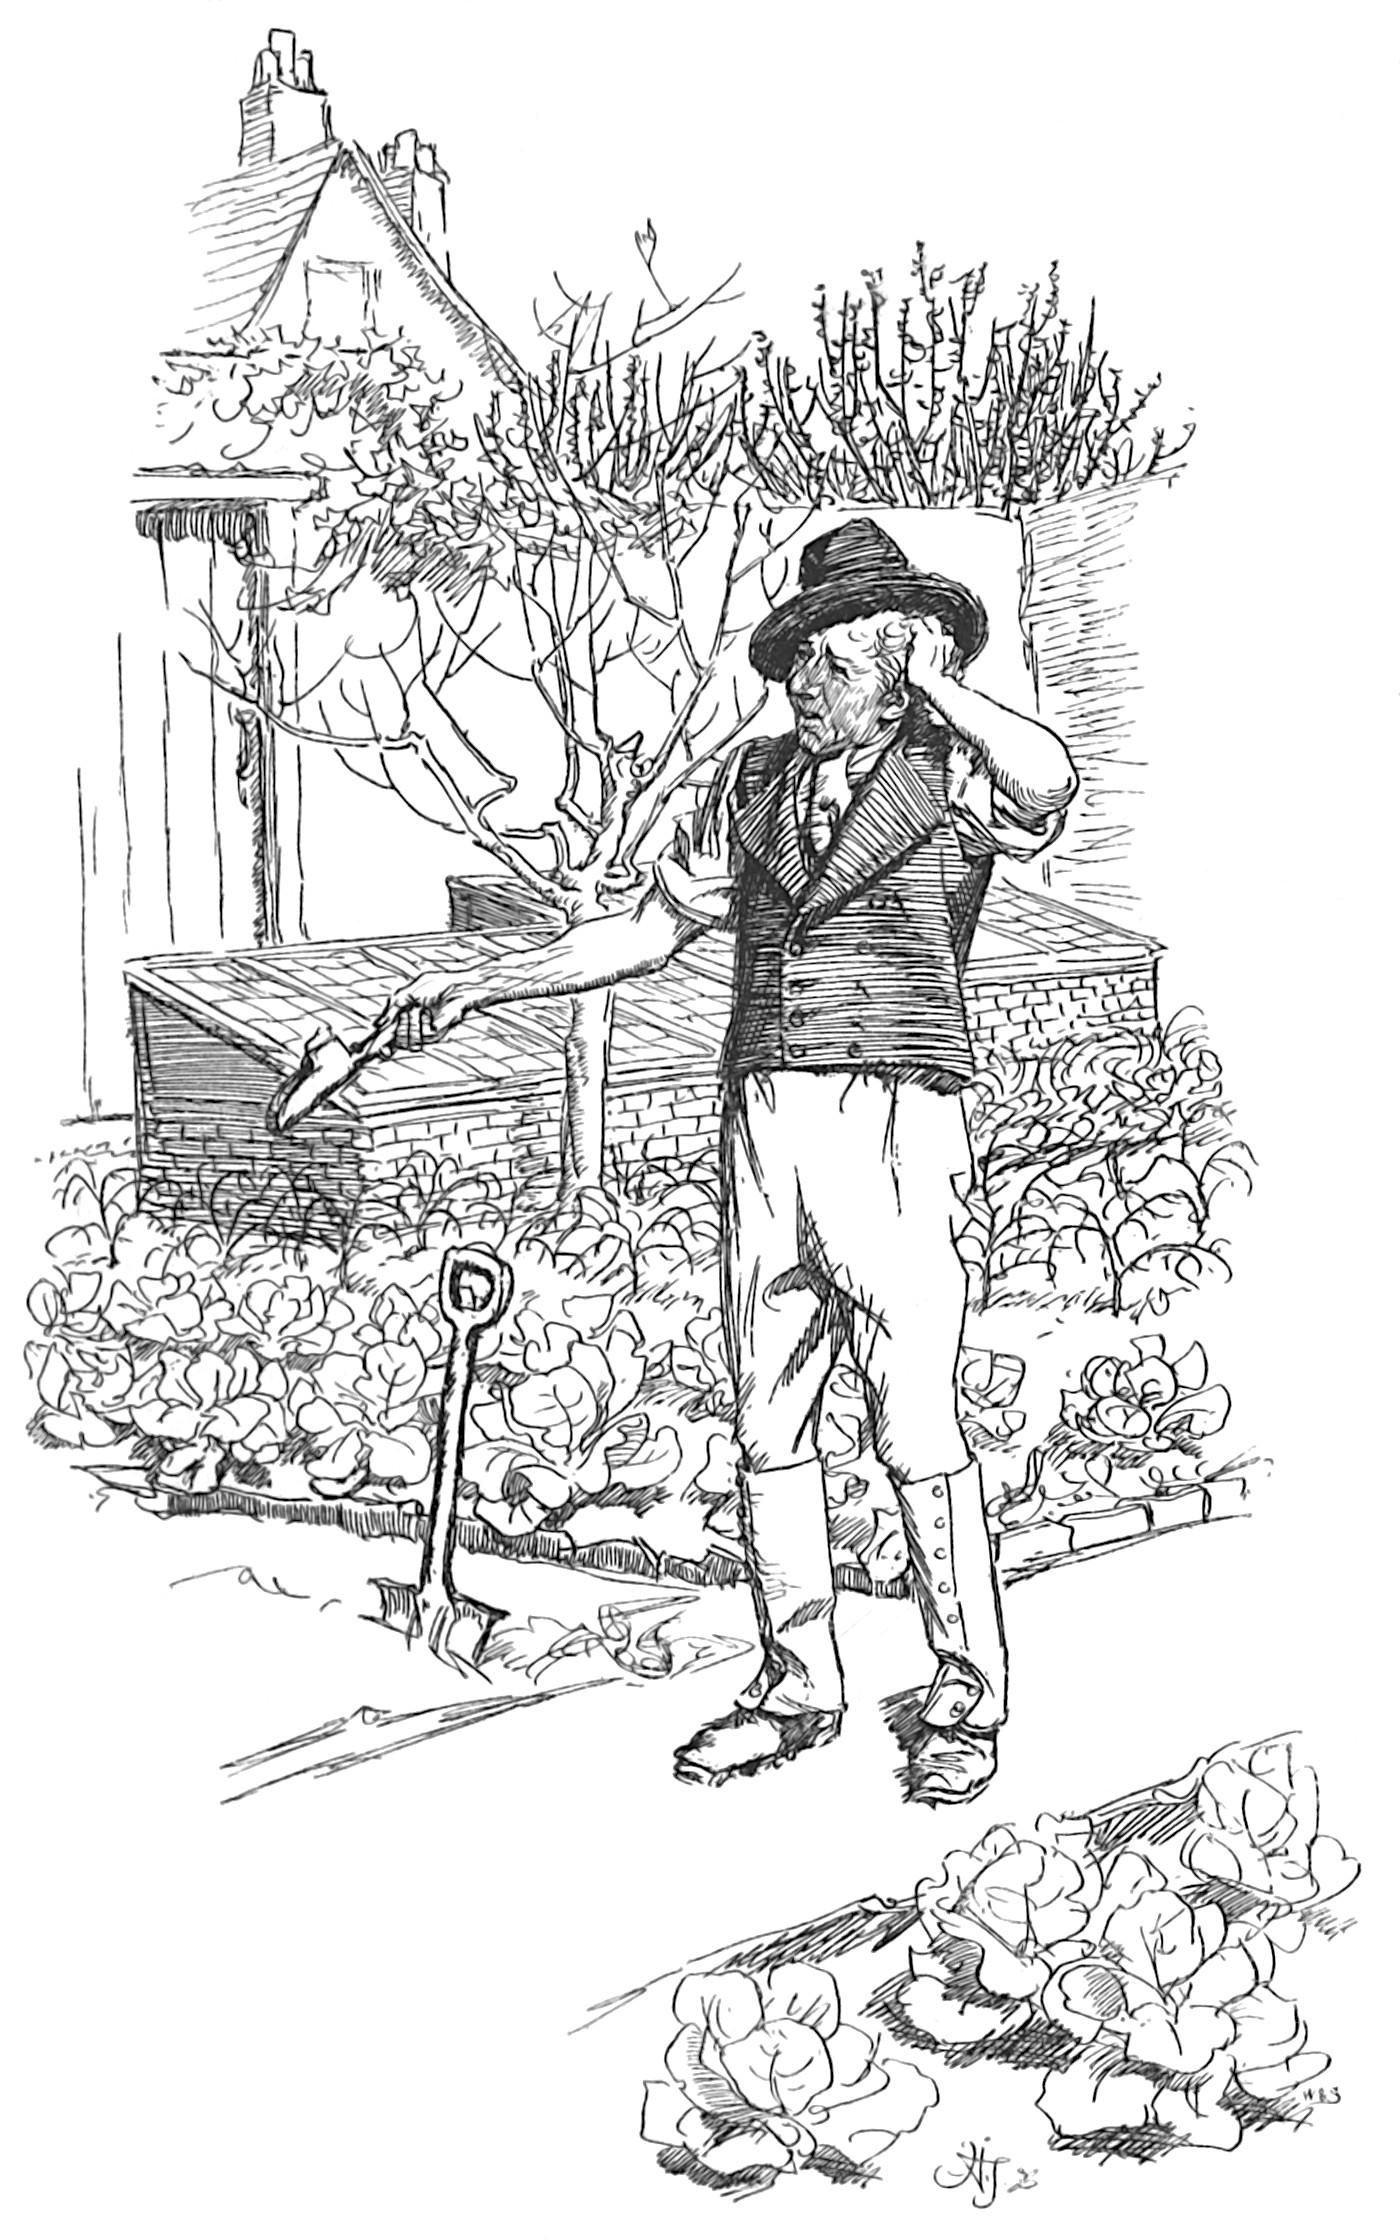
\includegraphics[width=.9\linewidth]{42lament}
		\caption{The gardener’s lamentations}
	\end{figure}
\end{a4}

\begin{letter}
	\begin{figure}[tbph]
		\centering
		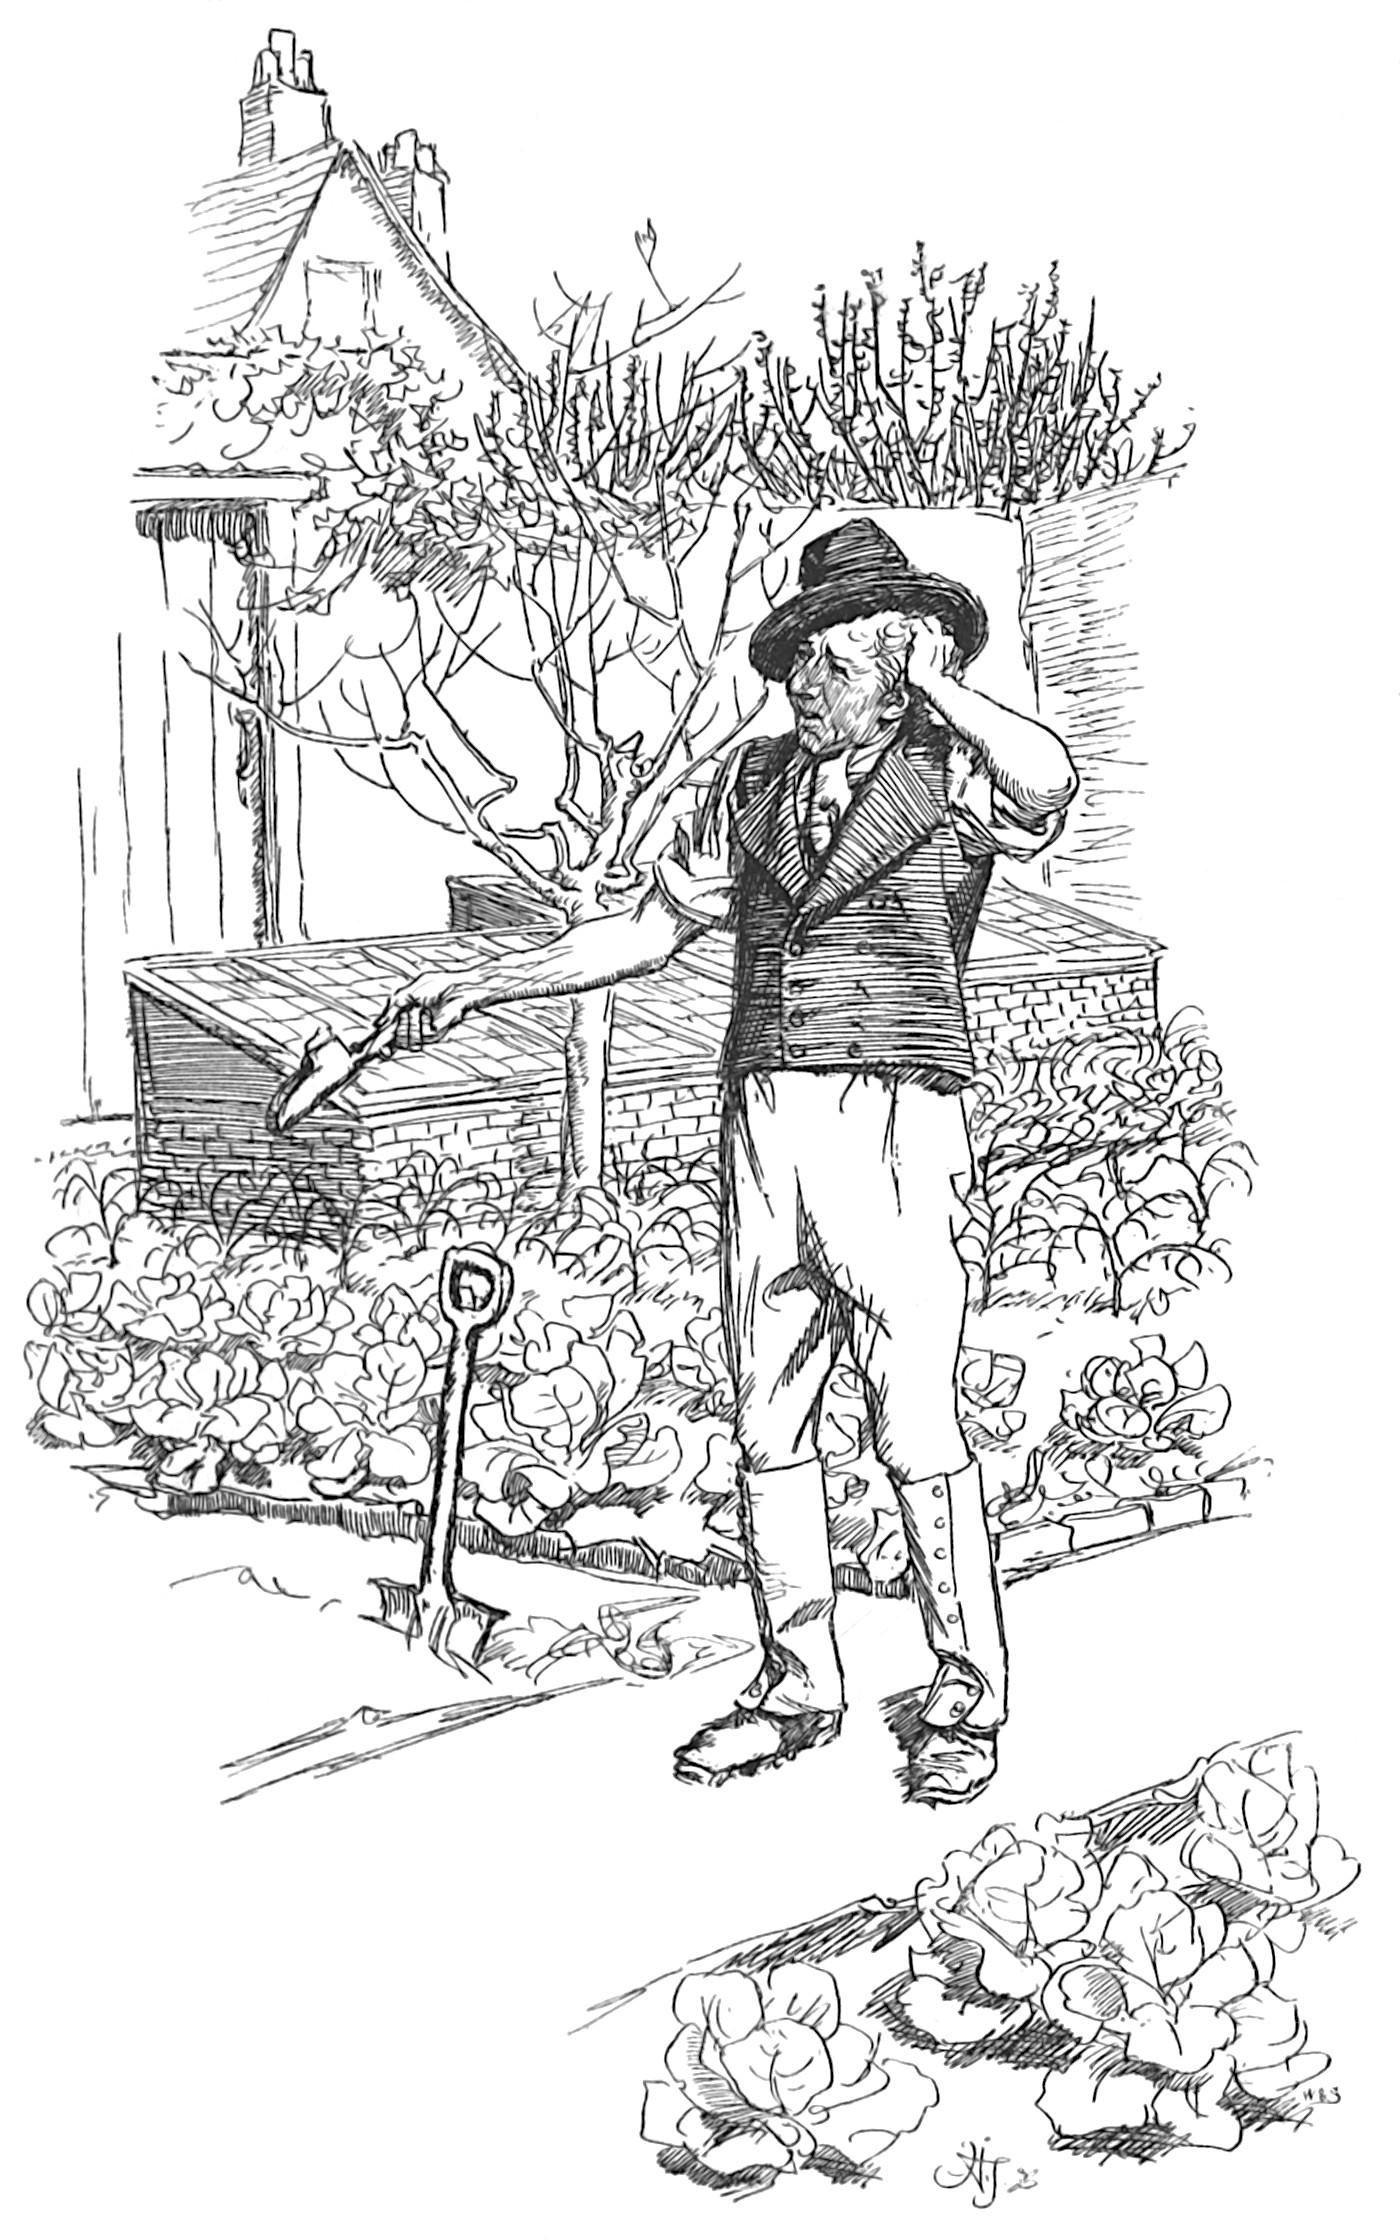
\includegraphics[width=\linewidth]{42lament}
		\caption{The gardener’s lamentations}
	\end{figure}
\end{letter}


The morning was fine and dry, and Marianne, in her plan of employment abroad, had not calculated for any change of weather during their stay at Cleveland. With great surprise therefore, did she find herself prevented by a settled rain from going out again after dinner. She had depended on a twilight walk to the Grecian temple, and perhaps all over the grounds, and an evening merely cold or damp would not have deterred her from it; but a heavy and settled rain even \textit{she} could not fancy dry or pleasant weather for walking.

Their party was small, and the hours passed quietly away. Mrs Palmer had her child, and Mrs Jennings her carpet-work; they talked of the friends they had left behind, arranged Lady Middleton’s engagements, and wondered whether Mr Palmer and Colonel Brandon would get farther than Reading that night. Elinor, however little concerned in it, joined in their discourse; and Marianne, who had the knack of finding her way in every house to the library, however it might be avoided by the family in general, soon procured herself a book.

Nothing was wanting on Mrs Palmer’s side that constant and friendly good humour could do, to make them feel themselves welcome. The openness and heartiness of her manner more than atoned for that want of recollection and elegance which made her often deficient in the forms of politeness; her kindness, recommended by so pretty a face, was engaging; her folly, though evident was not disgusting, because it was not conceited; and Elinor could have forgiven every thing but her laugh.

The two gentlemen arrived the next day to a very late dinner, affording a pleasant enlargement of the party, and a very welcome variety to their conversation, which a long morning of the same continued rain had reduced very low.

Elinor had seen so little of Mr Palmer, and in that little had seen so much variety in his address to her sister and herself, that she knew not what to expect to find him in his own family. She found him, however, perfectly the gentleman in his behaviour to all his visitors, and only occasionally rude to his wife and her mother; she found him very capable of being a pleasant companion, and only prevented from being so always, by too great an aptitude to fancy himself as much superior to people in general, as he must feel himself to be to Mrs Jennings and Charlotte. For the rest of his character and habits, they were marked, as far as Elinor could perceive, with no traits at all unusual in his sex and time of life. He was nice in his eating, uncertain in his hours; fond of his child, though affecting to slight it; and idled away the mornings at billiards, which ought to have been devoted to business. She liked him, however, upon the whole, much better than she had expected, and in her heart was not sorry that she could like him no more;—not sorry to be driven by the observation of his Epicurism, his selfishness, and his conceit, to rest with complacency on the remembrance of Edward’s generous temper, simple taste, and diffident feelings.

Of Edward, or at least of some of his concerns, she now received intelligence from Colonel Brandon, who had been into Dorsetshire lately; and who, treating her at once as the disinterested friend of Mr Ferrars, and the kind confidante of himself, talked to her a great deal of the parsonage at Delaford, described its deficiencies, and told her what he meant to do himself towards removing them.—His behaviour to her in this, as well as in every other particular, his open pleasure in meeting her after an absence of only ten days, his readiness to converse with her, and his deference for her opinion, might very well justify Mrs Jennings’s persuasion of his attachment, and would have been enough, perhaps, had not Elinor still, as from the first, believed Marianne his real favourite, to make her suspect it herself. But as it was, such a notion had scarcely ever entered her head, except by Mrs Jennings’s suggestion; and she could not help believing herself the nicest observer of the two;—she watched his eyes, while Mrs Jennings thought only of his behaviour;—and while his looks of anxious solicitude on Marianne’s feeling, in her head and throat, the beginning of a heavy cold, because unexpressed by words, entirely escaped the latter lady’s observation;—\textit{she} could discover in them the quick feelings, and needless alarm of a lover.

Two delightful twilight walks on the third and fourth evenings of her being there, not merely on the dry gravel of the shrubbery, but all over the grounds, and especially in the most distant parts of them, where there was something more of wildness than in the rest, where the trees were the oldest, and the grass was the longest and wettest, had—assisted by the still greater imprudence of sitting in her wet shoes and stockings—given Marianne a cold so violent as, though for a day or two trifled with or denied, would force itself by increasing ailments on the concern of every body, and the notice of herself. Prescriptions poured in from all quarters, and as usual, were all declined. Though heavy and feverish, with a pain in her limbs, and a cough, and a sore throat, a good night’s rest was to cure her entirely; and it was with difficulty that Elinor prevailed on her, when she went to bed, to try one or two of the simplest of the remedies.